\chapter{Specifikacija programske potpore}
		
		\section{Funkcionalni zahtjevi}
	
	Aktori koji izravno komuniciraju sa sustavom mogu imati ulogu inicijatora ili sudionika.
	Inicijatori pokreću procese u sustavu, konkretno radi se o neregistriranom i registriranom korisniku, recenzentu, organizatoru konferencije i administratoru. S druge strane, sudionici obavljaju određene poslove, konkretno radi se o bazi podataka.
	\newline
	
	
	
	
	\noindent \textbf{Dionici:}
	
	\begin{packed_enum}
		
		\item Organizator konferencije
		\item Sudionik konferencije
		\item Recenzent
		\item Administrator
		\item Razvojni tim
		
	\end{packed_enum}
	
	\noindent \textbf{Aktori i njihovi funkcionalni zahtjevi:}
	
	
	\begin{packed_enum}
		
			\item  \underbar{Organizator konferencije (inicijator) može:}
		\begin{packed_enum}
			
			\item pregledati sve podatke o sudionicima te ih mijenjati i dodavati sadržaj
			\item sudionicima slati obavijesti na njihove adrese elektroničke pošte
			\item pohraniti na lokalno računalo sve pristigle radove
			
		\end{packed_enum}
		
		\item  \underbar{Registrirani korisnik (inicijator) može:}
		\begin{packed_enum}
			
			\item obaviti prijavu u sustav
			\item pregledati sve definirane konferencije i njihove sekcije
			\item odabrati sekciju u kojoj želi sudjelovati i obaviti prijavu na sekciju
			\item pohraniti i uređivati vlastiti rad
			\item pregledati i uređivati osobne podatke
			\item prijaviti se za recenzenta konferencije
			\item izbrisati svoj korisnički račun
			
		\end{packed_enum}
		
		\item  \underbar{Administrator (inicijator) može:}
		
		\begin{packed_enum}
			
			\item upisati podatke o konferenciji i odrediti organizatora konferencije
			\item pregledati i izmijeniti podatke registriranog korisnika
			\item pohraniti sve dokumente koje su sudionici poslali
			i potvrdili kao konačnu inačicu
			\item pregledati statistiku vezanu za korisnike:
			\begin{packed_enum}
				
				\item broj trenutno prijavljenih korisnika
				\item ukupan broj i imena svih registriranih korisnika\newline
				
			\end{packed_enum}
				
		\end{packed_enum}
		
		
		\item  \underbar{Recenzent (inicijator) može:}
		\begin{packed_enum}
			
			\item pregledati prispjele radove svih sudionika konferencije
			\item definirati recenziju rada i odgovor na korisnikov zahtjev za sudjelovanjem na konferenciji: 
			\begin{packed_enum}
				
				\item prihvaćanjem rada
				\item prihvaćanjem rada, ali uz potrebnu doradu u manjoj mjeri
				(nije potrebna naknadna provjera)
				\item prihvaćanjem rada, ali uz potrebnu doradu u većoj mjeri
				(potrebna naknadna provjera)
				\item odbijanjem rada uz navođenje valjanog razloga
				
			\end{packed_enum}
			
			
		\end{packed_enum}
	
			\item  \underbar{Neregistrirani/neprijavljeni korisnik (inicijator) može:}
		\begin{packed_enum}
			
			\item obaviti registraciju u sustav, stvoriti novi korisnički račun za koji su mu potrebni ime, prezime, naziv institucije ili poduzeća u kojem djeluje, adresa boravka i adresa elektroničke pošte 
			
		\end{packed_enum}
		
		\item  \underbar{Baza podataka (sudionik):}
		
		\begin{packed_enum}
			
			\item pohranjuje podatke o svim korisnicima i njihovim ovlastima
			\item pohranjuje sve podatke o konferencijama, njihovim sekcijama i prispjelim radovima
			
			
		\end{packed_enum}
		
	
	\end{packed_enum}
	
	\eject 
	
			
			
				
			\subsection{Obrasci uporabe}
			
				
				\subsubsection{Opis obrazaca uporabe}
					

					\noindent \underbar{\textbf{UC1 - Registracija u sustav}}
					\begin{packed_item}
	
						\item \textbf{Glavni sudionik: }Neregistrirani korisnik
						\item  \textbf{Cilj:} Stvaranje korisničkog računa za pristup sustavu
						\item  \textbf{Sudionici:} Baza podataka
						\item  \textbf{Preduvjet:} -
						\item  \textbf{Opis osnovnog tijeka:}
						
						\item[] \begin{packed_enum}
							
							\item Korisnik odabire opciju za registraciju u sustav
							\item Korisnik unosi svoje podatke
							\item Korisniku se pridjeljuje njegova identifikacija
							\item Generira se lozinka koja se šalje korisniku
							\item Sustav šalje korisniku poveznicu za potvrdu registracije
							
						\end{packed_enum}
						
						\item  \textbf{Opis mogućih odstupanja:}
						
						\item[] \begin{packed_item}
	
							\item[2.a] Odabir već zauzetog korisničkog imena i/ili e-maila, unos korisničkih podataka u nedozvoljenom formatu ili pružanje neispravnog e-maila
							\item[] \begin{packed_enum}
								
								\item Sustav obavještava korisnika o neuspjelom upisu i vraća ga na stranicu za registraciju
								\item Korisnik mijenja potrebne podatke te završava unos ili odustaje od registracije
								
							\end{packed_enum}
						\end{packed_item}
					\end{packed_item}
				
				\noindent \underbar{\textbf{UC1.1 - Potvrdi registraciju}}
				\begin{packed_item}
					
					\item \textbf{Glavni sudionik: }Neregistrirani korisnik
					\item  \textbf{Cilj:} Potvrditi svoju registraciju u sustav
					\item  \textbf{Sudionici:} Baza podataka
					\item  \textbf{Preduvjet:} Ispunjen obrazac za uporabu
					\item  \textbf{Opis osnovnog tijeka:}
					
					\item[] \begin{packed_enum}
						
						\item Korisnik e-mailom prima poveznicu za potvrdu registracije
						\item Korisnik klikom na poveznicu potvrđuje stvaranje korisničkog računa
						\item Korisnikovi podatci se pohranjuju u bazu podataka
					
					\end{packed_enum}
					
					\item  \textbf{Opis mogućih odstupanja:}
					
					\item[] \begin{packed_item}
						
						\item[2.a] Korisnik ne potvrđuje svoju prijavu klikom na dobivenu poveznicu
						
						\item[] \begin{packed_enum}
							
							\item Registracija se ne potvrđuje\newline
							
						\end{packed_enum}
					\end{packed_item}
				\end{packed_item}
				
				\noindent \underbar{\textbf{UC2 - Pregled konferencija}}
				\begin{packed_item}
					
					\item \textbf{Glavni sudionik: }Registrirani korisnik
					\item  \textbf{Cilj:} Pregledati popis svih konferencija
					\item  \textbf{Sudionici:} Baza podataka
					\item  \textbf{Preduvjet:} Korisnik je prijavljen
					\item  \textbf{Opis osnovnog tijeka:}
					
					\item[] \begin{packed_enum}
						
						\item Korisnik odabire opciju "Pregledaj konferencije"
						\item Korisniku se prikazuju sve postojeće konferencije
						\item Korisnik odabire jednu od konferencija
						\item Prikazuju se informacije o konferenciji
						
					\end{packed_enum}
				\end{packed_item}
			
			\noindent \underbar{\textbf{UC3 - Prijava u sustav}}
			\begin{packed_item}
				
				\item \textbf{Glavni sudionik: }Registrirani korisnik
				\item  \textbf{Cilj:} Dobiti pristup početnom korisničkom sučelju i korisničkim funkcijama
				\item  \textbf{Sudionici:} Baza podataka
				\item  \textbf{Preduvjet:} Sudionik je registriran
				\item  \textbf{Opis osnovnog tijeka:}
				
				\item[] \begin{packed_enum}
					
					\item Korisnik izabire opciju "Prijava"
					\item Korisnik unosi svoj e-mail i lozinku
					\item Potvrda o ispravnosti unesenih podataka
					\item Pristup korisničkim funkcijama
					
				\end{packed_enum}
				
				\item  \textbf{Opis mogućih odstupanja:}
				
				\item[] \begin{packed_item}
					
					\item[3.a] Neispravno korisničko ime ili lozinka
					
					\item[] \begin{packed_enum}
						
						\item Sustav obavještava korisnika o neuspjeloj prijavi i vraća ga na stranicu za prijavu
						
					\end{packed_enum}
				\end{packed_item}
			\end{packed_item}
		
		\noindent \underbar{\textbf{UC3.1 - Generiranje nove lozinke}}
		\begin{packed_item}
			
			\item \textbf{Glavni sudionik: }Registrirani korisnik
			\item  \textbf{Cilj:} Dobiti novu lozinku na e-mail
			\item  \textbf{Sudionici:} Baza podataka
			\item  \textbf{Preduvjet:} Sudionik je registriran
			\item  \textbf{Opis osnovnog tijeka:}
			
			\item[] \begin{packed_enum}
				
				\item Korisnik odabire opciju "Zaboravljena lozinka"
				\item Korisnik u polje unosi svoju e-mail adresu
				\item Korisnik odabire gumb "Pošalji novu lozinku"
				\item Korisniku na e-mail dolazi nova lozinka za njegov račun
				
			\end{packed_enum}
			
			\item  \textbf{Opis mogućih odstupanja:}
			
			\item[] \begin{packed_item}
				
				\item[2.a] Neispravno unesena e-mail adresa
				
				\item[] \begin{packed_enum}
					
					\item Sustav obavještava korisnika da provjeri unesenu adresu
					
				\end{packed_enum}
			\end{packed_item}
		\end{packed_item}
	
	\noindent \underbar{\textbf{UC4 - Prijava za sudjelovanje na konferenciji}}
	\begin{packed_item}
		
		\item \textbf{Glavni sudionik: }Registrirani korisnik
		\item  \textbf{Cilj:} Prijaviti se na željenu konferenciju
		\item  \textbf{Sudionici:} Baza podataka
		\item  \textbf{Preduvjet:} Korisnik je prijavljen, postoje definirane konferencije
		\item  \textbf{Opis osnovnog tijeka:}
		
		\item[] \begin{packed_enum}
			
			\item  Korisnik bira opciju "Prijava za sudjelovanje na konferenciji"
			\item Korisniku se prikazuje lista svih postojećih konferencija
			\item Korisnik odabire konferenciju
			\item Korisniku se prikazuju informacije o konferenciji i popis sekcija
			\item Korisnik izabire opciju "Prijavi se"
			\item Korisniku se otvara obrazac za prijavu kojeg popunjava
			\item Korisnik potvrđuje prijavu
			
		\end{packed_enum}
	\end{packed_item}

	\noindent \underbar{\textbf{UC4.1 - Odabir sekcije}}
	\begin{packed_item}
		
		\item \textbf{Glavni sudionik: }Registrirani korisnik
		\item  \textbf{Cilj:} Odabrati sekciju unutar konferencije
		\item  \textbf{Sudionici:} Baza podataka
		\item  \textbf{Preduvjet:} Korisnik je prijavljen, nije prošao datum za prijavu u sekciju
		\item  \textbf{Opis osnovnog tijeka:}
		
		\item[] \begin{packed_enum}
			
			\item  Korisniku je prikazana lista sekcija koje može odabrati
			\item Korisnik odabire željenu sekciju
			
		\end{packed_enum}
	\end{packed_item}

	\noindent \underbar{\textbf{UC4.2 - Slanje potvrde o uspješnoj prijave}}
	\begin{packed_item}
		
		\item \textbf{Glavni sudionik: }Registrirani korisnik
		\item  \textbf{Cilj:} Dobiti odobrenje za sudjelovanje na konferenciji
		\item  \textbf{Sudionici:} Baza podataka
		\item  \textbf{Preduvjet:} Korisnik je prijavljen
		\item  \textbf{Opis osnovnog tijeka:}
		
		\item[] \begin{packed_enum}
			
			\item  Korisnik na e-mail dobiva potvrdu za sudjelovanje u sekciji
			\item Određuje se vrijeme unutar kojeg korisnik mora učitati svoj rad
			
		\end{packed_enum}
	\end{packed_item}

	\noindent \underbar{\textbf{UC4.3 - Učitavanje rada}}
	\begin{packed_item}
		
		\item \textbf{Glavni sudionik: }Registrirani korisnik
		\item  \textbf{Cilj:} Učitati svoj rad
		\item  \textbf{Sudionici:} Baza podataka
		\item  \textbf{Preduvjet:} Korisnik je prijavljen u sustav; odobrena mu je prijava u sekciju; nije prošlo vrijeme za učitavanje rada
		\item  \textbf{Opis osnovnog tijeka:}
		
		\item[] \begin{packed_enum}
			
			\item  Korisnik odabire opciju "Učitaj svoj rad"
			\item Korisniku se otvara polje u koje može učitati rad
			\item Korisnik odabire gumb "Pošalji" za slanje rada
			\item Sustav korisniku šalje obavijest o primitku rada
			
		\end{packed_enum}
		
		\item  \textbf{Opis mogućih odstupanja:}
		
		\item[] \begin{packed_item}
			
			\item[2.a] Korisnik je učitao datoteku koja nije u pdf formatu
			\item[] \begin{packed_enum} 
				\item Korisniku se javlja da je učitao datoteku pogrešnog formata
					\end{packed_enum}
				
			\item[2.b] Korisnik nije stisnuo gumb za slanje rada
			\item[] \begin{packed_enum}
				\item Sustav javlja korisniku da nije poslao učitani rad
				
			\end{packed_enum}
		\end{packed_item}
	\end{packed_item}

	\noindent \underbar{\textbf{UC5 - Pregled osobnih podataka}}
	\begin{packed_item}
		
		\item \textbf{Glavni sudionik: }Registrirani korisnik
		\item  \textbf{Cilj:} Pregledati osobne podatke
		\item  \textbf{Sudionici:} Baza podataka
		\item  \textbf{Preduvjet:} Korisnik je prijavljen
		\item  \textbf{Opis osnovnog tijeka:}
		
		\item[] \begin{packed_enum}
			
			\item  Korisnik odabire opciju za pregled osobnih podataka
			\item Sustav prikazuje osobne podatke korisnika
			
		\end{packed_enum}
	\end{packed_item}

	\noindent \underbar{\textbf{UC6 - Uređivanje osobnih podataka}}
	\begin{packed_item}
		
		\item \textbf{Glavni sudionik: }Registrirani korisnik
		\item  \textbf{Cilj:} Urediti osobne podatke
		\item  \textbf{Sudionici:} Baza podataka
		\item  \textbf{Preduvjet:} Korisnik je prijavljen
		\item  \textbf{Opis osnovnog tijeka:}
		
		\item[] \begin{packed_enum}
			
			\item  Korisnik odabire opciju za promjenu osobnih podataka
			\item Korisnik mijenja svoje podatke
			\item Korisnik sprema promjene
			\item Baza podataka se ažurira
			
		\end{packed_enum}
		
		\item  \textbf{Opis mogućih odstupanja:}
		
		\item[] \begin{packed_item}
			
			\item[2.a] Korisnik promijeni osobne podatke, ali ne odabire opciju "Spremi promjene"
			\item[] \begin{packed_enum}
				
				\item Sustav obavještava korisnika da nije spremio podatke prije izlaska iz prozora
				
			\end{packed_enum}
		\end{packed_item}
	\end{packed_item}

	\noindent \underbar{\textbf{UC7 - Brisanje korisničkog računa}}
	\begin{packed_item}
		
		\item \textbf{Glavni sudionik: }Registrirani korisnik
		\item  \textbf{Cilj:} Izbrisati svoj korisnički račun
		\item  \textbf{Sudionici:} Baza podataka
		\item  \textbf{Preduvjet:} Korisnik je prijavljen
		\item  \textbf{Opis osnovnog tijeka:}
		
		\item[] \begin{packed_enum}
			
			\item  Korisnik odabire pregled osobnih podataka
			\item Otvara se stranica s osobnim podatcima
			\item Korisnik bira opciju za brisanje računa
			\item Korisnički račun se briše iz baze podataka
			\item Otvara se stranica za registraciju
			
		\end{packed_enum}
	\end{packed_item}

	\noindent \underbar{\textbf{UC8 - Prijava za recenziranje}}
	\begin{packed_item}
		
		\item \textbf{Glavni sudionik: }Registrirani korisnik
		\item  \textbf{Cilj:} Prijaviti se za ulogu recenzenta
		\item  \textbf{Sudionici:} Baza podataka
		\item  \textbf{Preduvjet:} Korisnik je prijavljen
		\item  \textbf{Opis osnovnog tijeka:}
		
		\item[] \begin{packed_enum}
			
			\item  Korisnik izabire opciju "Prijavi se za recenziranje"
			\item Korisniku se otvara obrazac za prijavu
			\item Korisnik ispunjava obrazac za prijavu i potvrđuje ga
			\item Nakon potvrde organizatora korisnik dobiva ovlasti recenzenta
			
		\end{packed_enum}
		
		\item  \textbf{Opis mogućih odstupanja:}
		
		\item[] \begin{packed_item}
			
			\item[4.a] Organizator konferencije odbija prijavu za recenziranje
			\item[] \begin{packed_enum}
				
				\item Korisnik dobiva obavijest o neuspješnoj potvrdi prijave
				
			\end{packed_enum}
		\end{packed_item}
	\end{packed_item}

	\noindent \underbar{\textbf{UC9 - Uredi učitani rad}}
	\begin{packed_item}
		
		\item \textbf{Glavni sudionik: }Registrirani korisnik
		\item  \textbf{Cilj:} Urediti svoj učitani rad
		\item  \textbf{Sudionici:} Baza podataka
		\item  \textbf{Preduvjet:} Korisnik je prijavljen, rad je prethodno učitan
		\item  \textbf{Opis osnovnog tijeka:}
		
		\item[] \begin{packed_enum}
			
			\item Korisnik odabire opciju "Uredi rad"
			\item Sustav prikazuje sve do tada predane radove
			\item Korisnik odabire rad koji želi urediti
			\item Korisnik uređuje rad
			\item Korisnik pohranjuje promjene
			\item Promjena se sprema u bazu podataka
		\end{packed_enum}
		
		\item  \textbf{Opis mogućih odstupanja:}
		
		\item[] \begin{packed_item}
			
			\item[2.a] Korisnik nema učitanih radova
			\item[] \begin{packed_enum}
				\item Sustav ispisuje poruku "Nema učitanih radova"
			
			\end{packed_enum}
	
			\item[4.a] Korisnik promijeni rad, ali ne odabire opciju "Spremi promjene"
			\item[] \begin{packed_enum}
				\item Sustav obavještava korisnika da nije spremio promjene prije izlaska iz prozora
			
			\end{packed_enum}
		\end{packed_item}
	\end{packed_item}

	\noindent \underbar{\textbf{UC10 - Pregledaj radove}}
	\begin{packed_item}
		
		\item \textbf{Glavni sudionik: }Recenzent
		\item  \textbf{Cilj:} Pregledati popis svih radova
		\item  \textbf{Sudionici:} Baza podataka
		\item  \textbf{Preduvjet:} Recenzent je prijavljen
		\item  \textbf{Opis osnovnog tijeka:}
		
		\item[] \begin{packed_enum}
			
			\item  Recenzent bira opciju "Pregledaj radove"
			\item Recenzentu se otvara popis svih učitanih radova
			
		\end{packed_enum}
		
		\item  \textbf{Opis mogućih odstupanja:}
		
		\item[] \begin{packed_item}
			
			\item[2.a] U sustav još nisu učitani radovi za odabranu sekciju
			\item[] \begin{packed_enum}
				
				\item Sustav ispisuje poruku "Nema radova"
				
			\end{packed_enum}
		\end{packed_item}
	\end{packed_item}

	\noindent \underbar{\textbf{UC11 - Prijava za sudjelovanje na konferenciji}}
	\begin{packed_item}
		
		\item \textbf{Glavni sudionik: }Recenzent
		\item  \textbf{Cilj:} Odbijanje rada
		\item  \textbf{Sudionici:} Baza podataka
		\item  \textbf{Preduvjet:} Recenzent je prijavljen, sudionik konferencije je učitao svoj rad
		\item  \textbf{Opis osnovnog tijeka:}
		
		\item[] \begin{packed_enum}
			
			\item  Recenzent bira opciju "Recenziraj rad"
			\item Recenzent bira ocjenu "Rad odbijen"
			\item Korisnik odabire konferenciju
			\item Recenzent unosi primjedbe u odgovarajuće polje
			\item Recenzent potvrđuje svoj odabir
			\item Sustav obavještava korisnika o odluci recenzenta
			
		\end{packed_enum}
	\end{packed_item}

	\noindent \underbar{\textbf{UC12 - Prihvati rad}}
	\begin{packed_item}
		
		\item \textbf{Glavni sudionik: }Recenzent
		\item  \textbf{Cilj:} Prihvatiti rad bez izmjena
		\item  \textbf{Sudionici:} Baza podataka
		\item  \textbf{Preduvjet:} Recenzent je prijavljen, sudionik konferencije je učitao svoj rad
		\item  \textbf{Opis osnovnog tijeka:}
		
		\item[] \begin{packed_enum}
			
			\item  Recenzent bira opciju "Recenziraj rad"
			\item Recenzent bira ocjenu "Rad prihvaćen"
			\item Recenzent potvrđuje svoj odabir
			\item Sustav obavještava korisnika o odluci recenzenta
			
		\end{packed_enum}
	\end{packed_item}

	\noindent \underbar{\textbf{UC13 - Prihvati rad uz izmjene}}
	\begin{packed_item}
		
		\item \textbf{Glavni sudionik: }Recenzent
		\item  \textbf{Cilj:} Izabrati željenu konferenciju
		\item  \textbf{Sudionici:} Baza podataka
		\item  \textbf{Preduvjet:} Recenzent je prijavljen, sudionik konferencije je učitao svoj rad
		\item  \textbf{Opis osnovnog tijeka:}
		
		\item[] \begin{packed_enum}
			
			\item Recenzent bira opciju "Recenziraj rad"
			\item Recenzent bira ocjenu "Rad prihvaćen uz izmjene"
			\item Recenzent unosi primjedbe u odgovarajuće polje
			\item Recenzent potvrđuje svoj odabir
			\item Sustav obavještava korisnika o odluci recenzenta
			
		\end{packed_enum}
	\end{packed_item}

	\noindent \underbar{\textbf{UC14 - Preuzmi rad lokalno}}
	\begin{packed_item}
		
		\item \textbf{Glavni sudionik: }Recenzent
		\item  \textbf{Cilj:} Preuzeti rad na svoje računalo
		\item  \textbf{Sudionici:} Baza podataka
		\item  \textbf{Preduvjet:} Recenzent je prijavljen, sudionik konferencije je učitao svoj rad
		\item  \textbf{Opis osnovnog tijeka:}
		
		\item[] \begin{packed_enum}
			
			\item Recenzent bira opciju "Preuzmi rad na računalo"
			\item Na računalo recenzenta se sprema rad u pdf formatu
			
		\end{packed_enum}
	\end{packed_item}

	\noindent \underbar{\textbf{UC15 - Pregledaj rad online}}
	\begin{packed_item}
		
		\item \textbf{Glavni sudionik: }Recenzent
		\item  \textbf{Cilj:} Pregledati rad online
		\item  \textbf{Sudionici:} Baza podataka
		\item  \textbf{Preduvjet:} Recenzent je prijavljen, sudionik konferencije je učitao svoj rad
		\item  \textbf{Opis osnovnog tijeka:}
		
		\item[] \begin{packed_enum}
			
			\item  Recenzent bira opciju "Pregledaj rad online"
			\item Rad se prikazuje u novoj kartici preglednika
			
		\end{packed_enum}
	\end{packed_item}

	\noindent \underbar{\textbf{UC16 - Odobri prijavu za recenziranje}}
	\begin{packed_item}
		
		\item \textbf{Glavni sudionik: }Organizator konferencije
		\item  \textbf{Cilj:} Odobriti zahtjev za recenziranje radova
		\item  \textbf{Sudionici:} Baza podataka
		\item  \textbf{Preduvjet:} Organizator je prijavljen
		\item  \textbf{Opis osnovnog tijeka:}
		
		\item[] \begin{packed_enum}
			
			\item Organizator konferencije odabire opciju "Zahtjevi za recenziranje"
			\item Sustav prikazuje popis primljenih zahtjeva za recenziranje
			\item Organizator konferencije odobrava ili odbacuje zahtjev
			\item Prijavljenog se obavještava o potvrđenoj prijavi
			
		\end{packed_enum}
		
		\item  \textbf{Opis mogućih odstupanja:}
		
		\item[] \begin{packed_item}
			
			\item[2.a] Nema primljenih zahtjeva za recenziranje
			\item[] \begin{packed_enum}
				
				\item Sustav ispisuje poruku "Nema pristiglih zahtjeva"
				
			\end{packed_enum}
		\end{packed_item}
	\end{packed_item}

	\noindent \underbar{\textbf{UC17 - Slanje obavijesti sudionicima}}
	\begin{packed_item}
		
		\item \textbf{Glavni sudionik: }Organizator konferencije
		\item  \textbf{Cilj:} Slanje obavijesti sudionicima
		\item  \textbf{Sudionici:} Baza podataka
		\item  \textbf{Preduvjet:} Organizator je prijavljen
		\item  \textbf{Opis osnovnog tijeka:}
		
		\item[] \begin{packed_enum}
			
			\item Organizator konferencije bira opciju "Pošalji obavijest sudionicima"
			\item Organizator konferencije upisuje obavijest u odgovarajuće polje
			\item Organizator odabire konferenciju među ponuđenima
			\item Sustav prikazuje popis svih sudionika za odabranu konferenciju
			\item Organizator konferencije bira opciju "Pošalji svima" ili odabire željene sudionike
			\item Potvrdom obavijesti ona se šalje sudionicima na e-mail
			
		\end{packed_enum}
		
		\item  \textbf{Opis mogućih odstupanja:}
		
		\item[] \begin{packed_item}
			
			\item[4.a] Na odabranoj konferenciji nema sudionika
			\item[] \begin{packed_enum}
				\item Sustav ispisuje poruku "Nema sudionika"
				
			\end{packed_enum}
			\item[6.a] Organizator sastavlja obavijest, ali napušta prozor bez potvrde slanja
			\item[] \begin{packed_enum}
				\item Sustav obavještava organizatora da slanje obavijesti nije potvrđeno
				
			\end{packed_enum}
		\end{packed_item}
	\end{packed_item}

	\noindent \underbar{\textbf{UC18 - Preuzmi rad sudionika}}
	\begin{packed_item}
		
		\item \textbf{Glavni sudionik: }Organizator konferencije
		\item  \textbf{Cilj:} Preuzeti pohranjeni rad sudionika konferencije
		\item  \textbf{Sudionici:} Baza podataka
		\item  \textbf{Preduvjet:} Organizator je prijavljen
		\item  \textbf{Opis osnovnog tijeka:}
		
		\item[] \begin{packed_enum}
			
			\item Organizator konferencije odabire opciju "Preuzmi rad sudionika"
			\item Prikazuje se popis svih radova po sekcijama
			\item Organizator odabire radove koje želi preuzeti
			\item Organizator potvrđuje odabir i radovi se preuzimaju
			
		\end{packed_enum}
		
		\item  \textbf{Opis mogućih odstupanja:}
		
		\item[] \begin{packed_item}
			
			\item[2.a] Nema učitanih radova na konfereniciji
			\item[] \begin{packed_enum}
				
				\item Sustav ispisuje poruku "Nema radova"
				
			\end{packed_enum}
		\end{packed_item}
	\end{packed_item}

	\noindent \underbar{\textbf{UC19 - Pregled statistike o radovima}}
	\begin{packed_item}
		
		\item \textbf{Glavni sudionik: }Organizator konferencije
		\item  \textbf{Cilj:} Pregledati broj radova ukupno i po sekcijama
		\item  \textbf{Sudionici:} Baza podataka
		\item  \textbf{Preduvjet:} Organizator je prijavljen
		\item  \textbf{Opis osnovnog tijeka:}
		
		\item[] \begin{packed_enum}
			
			\item Organizator odabire opciju "Pregledaj sve radove"
			\item Prikazuje se popis svih radova po sekcijama
			\item Organizator odabire opciju "Prikaži statistiku"
			\item Prikazuje se statistika za odabranu konferenciju
			
		\end{packed_enum}
	\end{packed_item}

	\noindent \underbar{\textbf{UC20 - Pregled podataka korisnika}}
	\begin{packed_item}
		
		\item \textbf{Glavni sudionik: }Administrator
		\item  \textbf{Cilj:} Pregledati podatke korisnika
		\item  \textbf{Sudionici:} Baza podataka
		\item  \textbf{Preduvjet:} Administrator je prijavljen
		\item  \textbf{Opis osnovnog tijeka:}
		
		\item[] \begin{packed_enum}
			
			\item Administrator bira opciju "Pregledaj podatke korisnika"
			\item Administrator konferencije pronalazi željenog sudionika
			\item Podatci korisnika se prikazuju
			
		\end{packed_enum}
		
		\item  \textbf{Opis mogućih odstupanja:}
		
		\item[] \begin{packed_item}
			
			\item[2.a] Nema registriranih korisnika
			\item[] \begin{packed_enum}
				
				\item Sustav ispisuje poruku "Nema registriranih korisnika"
				
			\end{packed_enum}
		\end{packed_item}
	\end{packed_item}

	\noindent \underbar{\textbf{UC21 - Mijenjanje podataka sudionika}}
	\begin{packed_item}
		
		\item \textbf{Glavni sudionik: }Administrator
		\item  \textbf{Cilj:} Promijeniti podatke sudioniku konferencije
		\item  \textbf{Sudionici:} Baza podataka
		\item  \textbf{Preduvjet:} Administrator je prijavljen
		\item  \textbf{Opis osnovnog tijeka:}
		
		\item[] \begin{packed_enum}
			
			\item Administrator bira opciju "Pregledaj podatke sudionika"
			\item Administrator pronalazi željenog sudionika
			\item Podatci korisnika se prikazuju
			\item Administrator bira opciju "Promijeni podatke"
			\item Administrator mijenja podatke sudioniku
			\item Administrator sprema promjene
			\item Baza podataka se ažurira
			
		\end{packed_enum}
		
		\item  \textbf{Opis mogućih odstupanja:}
		
		\item[] \begin{packed_item}
			
			\item[1.a] Nema registriranih korisnika
			\item[] \begin{packed_enum}
				\item Sustav ispisuje poruku "Nema registriranih korisnika"
				
			\end{packed_enum}
		
			\item[5.a] Organizator mijenja podatke, ali ne odabire opciju "Spremi promjene"
			\item[] \begin{packed_enum}
				\item Sustav obavještava organizatora da nije spremio podatke
				
			\end{packed_enum}
		\end{packed_item}
	\end{packed_item}

	\noindent \underbar{\textbf{UC22 - Dodavanje podataka sudioniku}}
	\begin{packed_item}
		
		\item \textbf{Glavni sudionik: }Administrator
		\item  \textbf{Cilj:} Dodati podatke sudioniku
		\item  \textbf{Sudionici:} Baza podataka
		\item  \textbf{Preduvjet:} Administrator je prijavljen
		\item  \textbf{Opis osnovnog tijeka:}
		
		\item[] \begin{packed_enum}
			
			\item Administrator bira opciju "Pregledaj podatke sudionika"
			\item Administrator pronalazi željenog sudionika
			\item Podatci korisnika se prikazuju
			\item Administrator bira opciju "Dodaj podatke"
			\item Administrator dodaje podatke sudioniku
			\item Administrator sprema promjene
			\item Baza podataka se ažurira
			
		\end{packed_enum}
		
		\item  \textbf{Opis mogućih odstupanja:}
		
		\item[] \begin{packed_item}
			
			\item[1.a] Nema registriranih korisnika
			\item[] \begin{packed_enum}
				\item Sustav ispisuje poruku "Nema registriranih korisnika"
				
			\end{packed_enum}
			
			\item[5.a] Organizator dodaje podatke, ali ne odabire opciju "Spremi promjene"
			\item[] \begin{packed_enum}
				\item Sustav obavještava organizatora da nije spremio podatke
				
			\end{packed_enum}
		\end{packed_item}
	\end{packed_item}

	\noindent \underbar{\textbf{UC23 - Pregled aktivnih korisnika}}
	\begin{packed_item}
		
		\item \textbf{Glavni sudionik: }Administrator
		\item  \textbf{Cilj:} Pregledati aktivne korisnike
		\item  \textbf{Sudionici:} Baza podataka
		\item  \textbf{Preduvjet:} Administrator je prijavljen
		\item  \textbf{Opis osnovnog tijeka:}
		
		\item[] \begin{packed_enum}
			
			\item Administrator odabire opciju "Popis aktivnih korisnika"
			\item Prikazuje se popis i broj korisnika koji su trenutno aktivni
			
		\end{packed_enum}
	\end{packed_item}

	\noindent \underbar{\textbf{UC24 - Stvaranje nove konferencije}}
	\begin{packed_item}
		
		\item \textbf{Glavni sudionik: }Administrator
		\item  \textbf{Cilj:} Stvoriti novu konferenciju
		\item  \textbf{Sudionici:} Baza podataka
		\item  \textbf{Preduvjet:} Administrator je prijavljen
		\item  \textbf{Opis osnovnog tijeka:}
		
		\item[] \begin{packed_enum}
			
			\item Administrator odabire opciju "Stvori novu konferenciju"
			\item Prikazuje se prozor za unos opcija
			\item Administrator popunjava opcije
			\item Administrator potvrđuje unesene podatke
			
		\end{packed_enum}
		
		\item  \textbf{Opis mogućih odstupanja:}
		
		\item[] \begin{packed_item}
			
			\item[1.a] Administrator dodaje podatke, ali ne odabire opciju "Spremi promjene"
			\item[] \begin{packed_enum}
				\item Sustav obavještava administratora da nije spremio podatke\newline\newline\newline
				
			\end{packed_enum}
		\end{packed_item}
	\end{packed_item}

	\noindent \underbar{\textbf{UC24.1 - Upisivanje podataka o konferenciji}}
	\begin{packed_item}
		
		\item \textbf{Glavni sudionik: }Administrator
		\item  \textbf{Cilj:} Upisati podatke za novu konferenciju
		\item  \textbf{Sudionici:} Baza podataka
		\item  \textbf{Preduvjet:} Administrator je prijavljen
		\item  \textbf{Opis osnovnog tijeka:}
		
		\item[] \begin{packed_enum}
			
			\item Administrator odabire opciju za unos podataka o konferenciji
			\item Administrator unosi sve potrebne podatke o konferenciji
			
		\end{packed_enum}
	\end{packed_item}

	\noindent \underbar{\textbf{UC24.2 - Odredi organizatora konferencije}}
	\begin{packed_item}
		
		\item \textbf{Glavni sudionik: }Administrator
		\item  \textbf{Cilj:} Odrediti organizatora nove konferencije
		\item  \textbf{Sudionici:} Baza podataka
		\item  \textbf{Preduvjet:} Administrator je prijavljen
		\item  \textbf{Opis osnovnog tijeka:}
		
		\item[] \begin{packed_enum}
			
			\item Administrator odabire opciju za dodavanje organizatora
			\item Administrator u sustavu odabire organizatora konferencije
			
		\end{packed_enum}
	\end{packed_item}

	\noindent \underbar{\textbf{UC24.3 - Definiranje upitnika za prijavu}}
	\begin{packed_item}
		
		\item \textbf{Glavni sudionik: }Administrator
		\item  \textbf{Cilj:} Definirati upitnik za prijavu na konferenciju
		\item  \textbf{Sudionici:} Baza podataka
		\item  \textbf{Preduvjet:} Administrator je prijavljen
		\item  \textbf{Opis osnovnog tijeka:}
		
		\item[] \begin{packed_enum}
			
			\item Administrator odabire opciju za definiranje upitnika za prijavu
			\item Administrator definira upitnik na temelju zahtjeva organizatora
			
		\end{packed_enum}
	\end{packed_item}
	
				\subsubsection{Dijagrami obrazaca uporabe}
				
				\begin{figure}[H]
					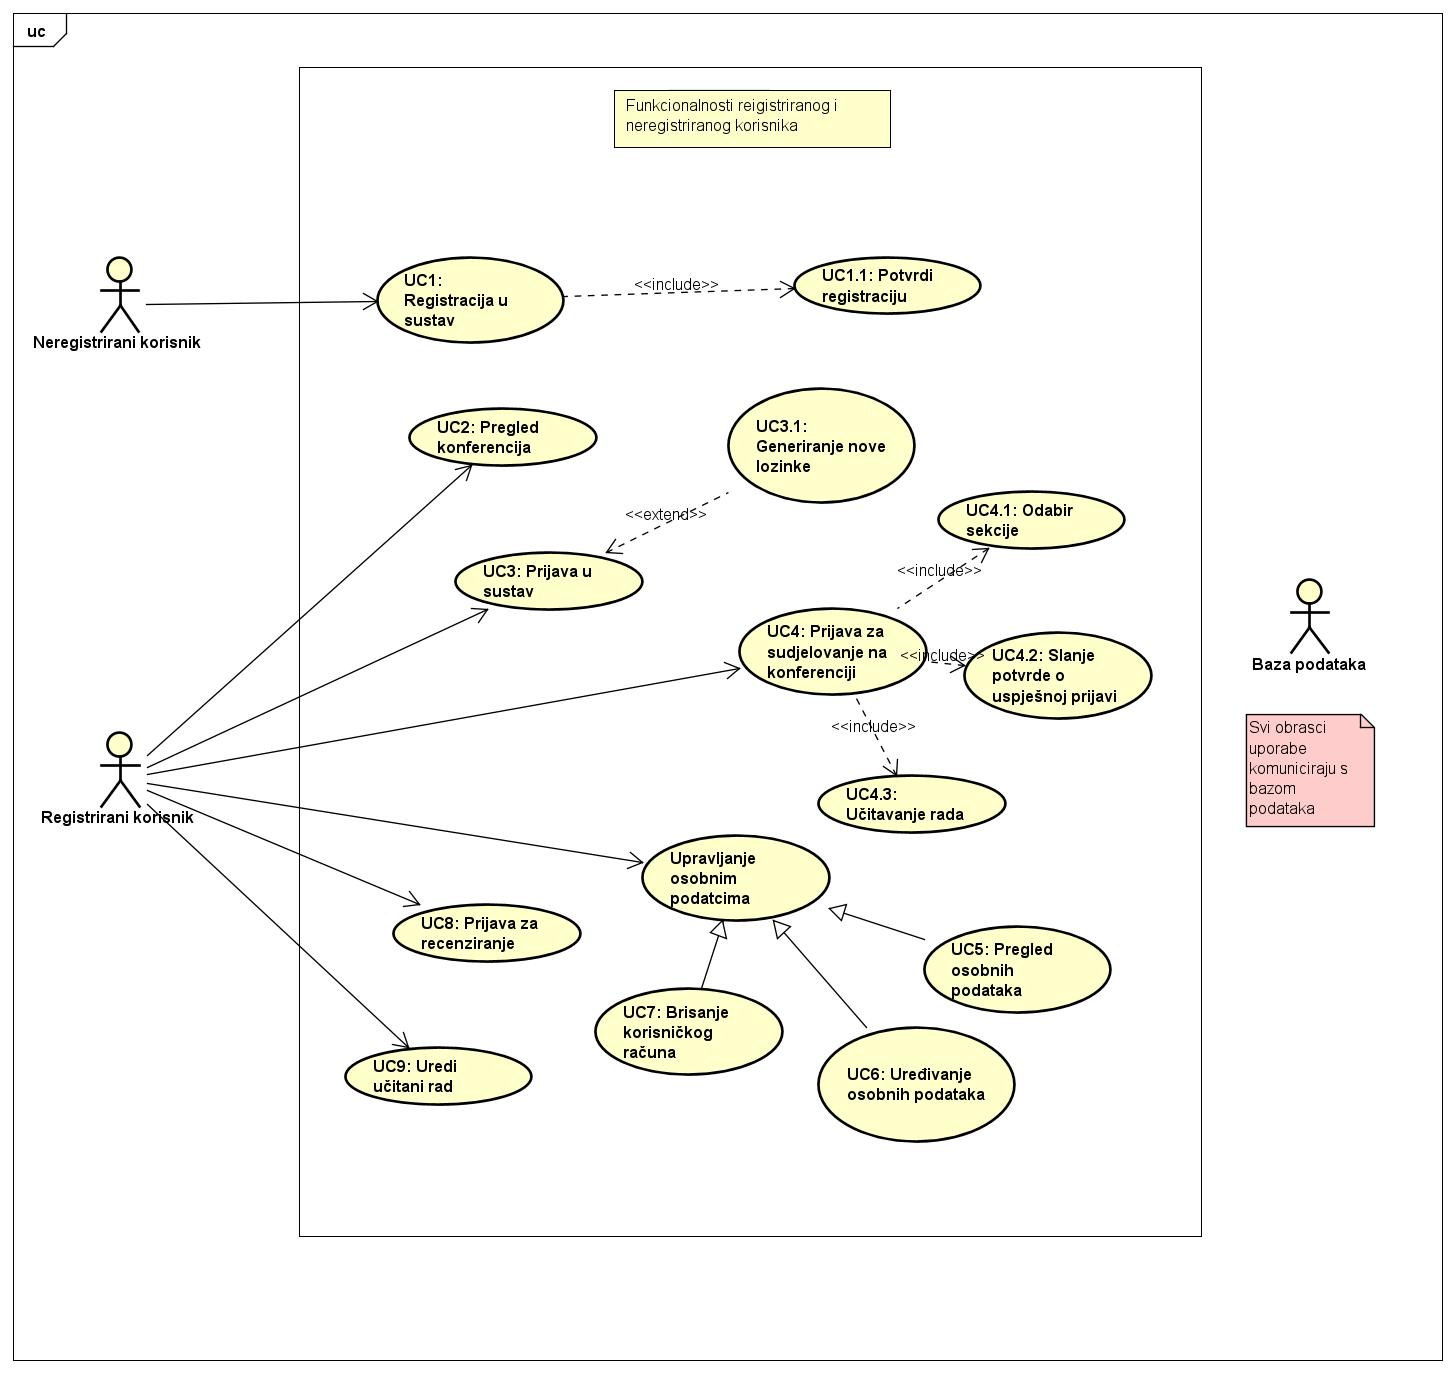
\includegraphics[width=1\linewidth]{slike/UCdijagram1} %veličina u odnosu na širinu linije
					\centering
					\caption{Dijagram obrasca uporabe, funkcionalnosti neregistriranog i registriranog korisnika}
					\label{fig:UC1} %label mora biti drugaciji za svaku sliku
				\end{figure}
			
				\begin{figure}[H]
					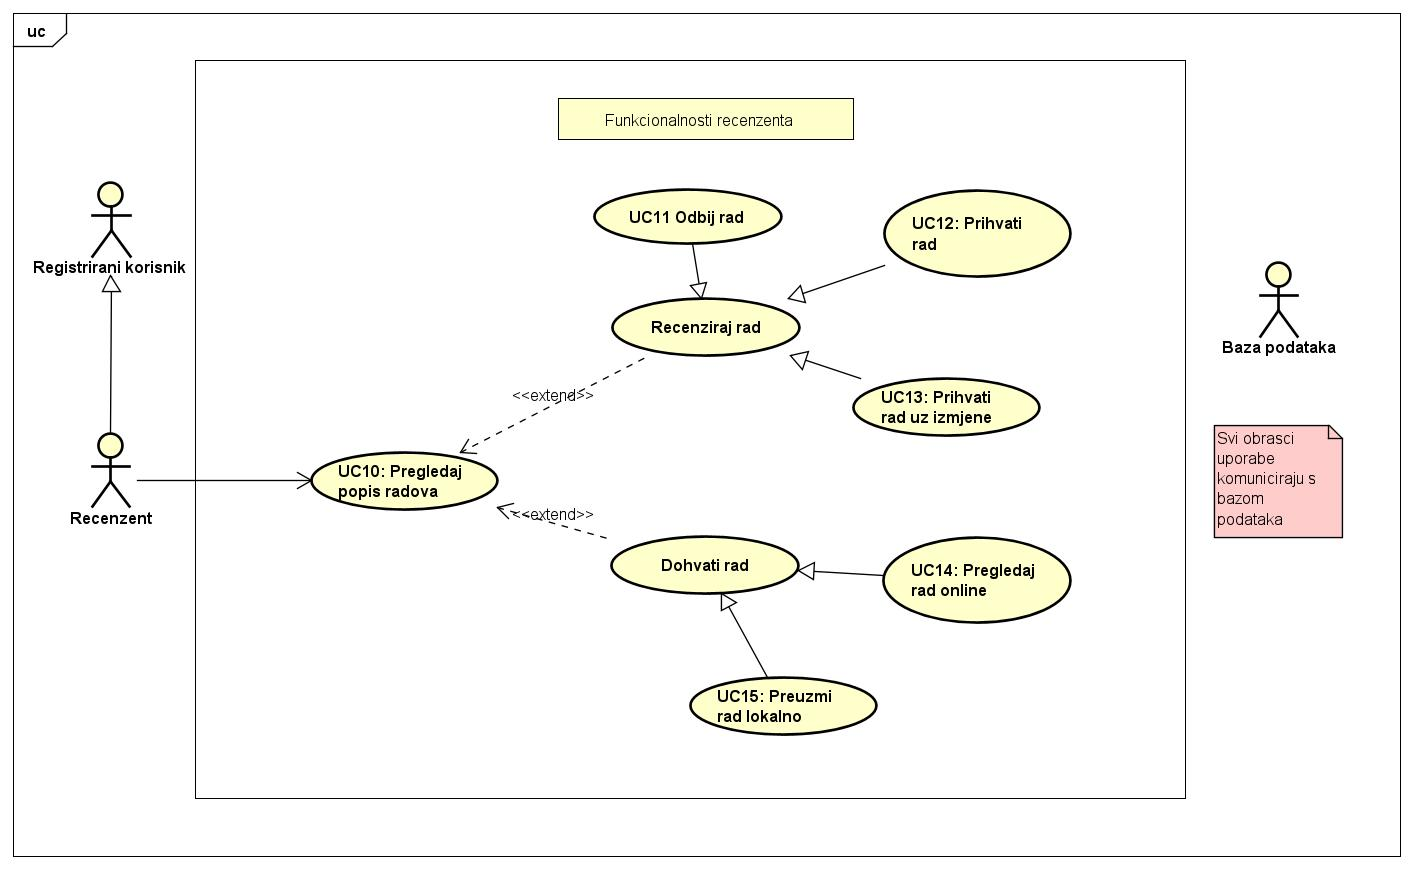
\includegraphics[width=1\linewidth]{slike/UCdijagram2} %veličina u odnosu na širinu linije
					\centering
					\caption{Dijagram obrasca uporabe, funkcionalnosti recenzenta}
					\label{fig:UC2} %label mora biti drugaciji za svaku sliku
				\end{figure}
				
				\begin{figure}[H]
					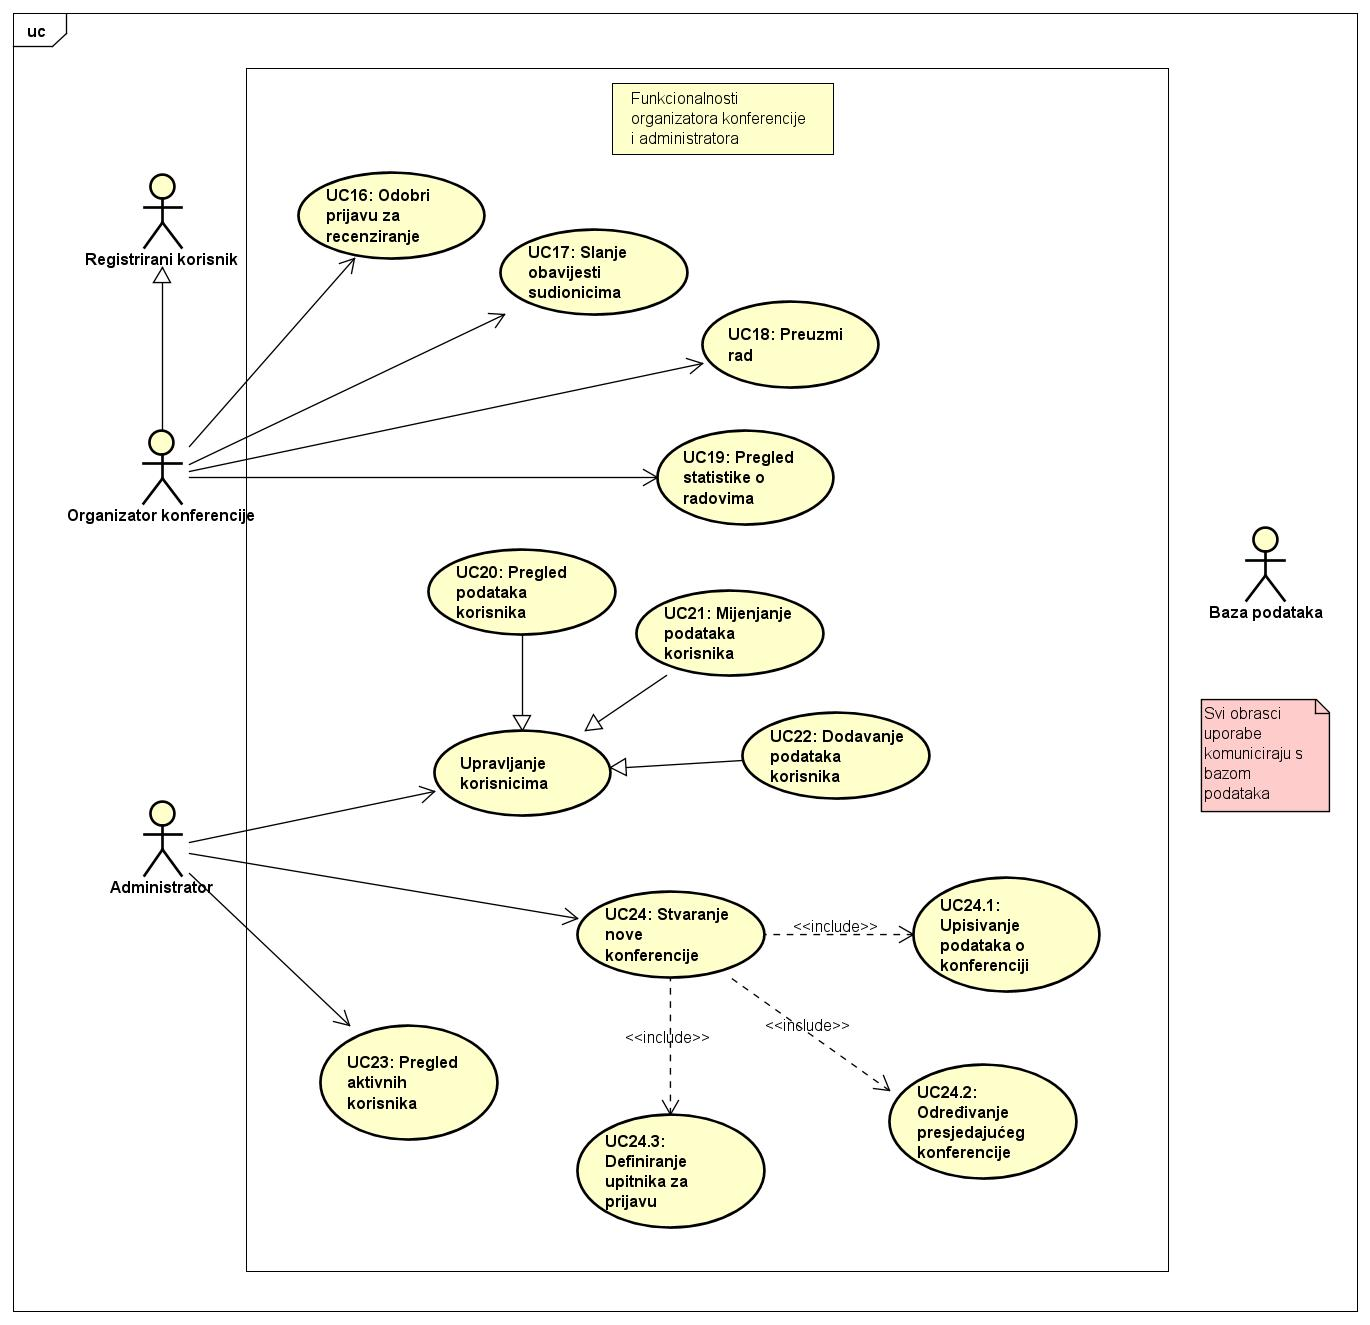
\includegraphics[width=1\linewidth]{slike/UCdijagram3} %veličina u odnosu na širinu linije
					\centering
					\caption{Dijagram obrasca uporabe, funkcionalnosti organizatora konferencije i administratora}
					\label{fig:UC3} %label mora biti drugaciji za svaku sliku
				\end{figure}
		
			\text\newline\newline\newline\newline\newline\newline
				
			\subsection{Sekvencijski dijagrami}

				
				\noindent\textbf{Obrazac uporabe UC6 - Uređivanje osobnih podataka}\\
				
				\noindent Korisnik odabire opciju za promjenu osobnih podataka. Poslužitelj iz baze podataka dohvaća osobne podatke korisnika postavljene pri obavljanju registracije u sustav i stvaranju korisničkog računa. Biranjem odabrane funkcionalnosti sustava i uspješnim dohvaćanjem osobnih podataka iz baze podataka korisnik dobiva pregled svih ranije definiranih osobnih podataka. Korisnik mijenja svoje podatke unošenjem novih vrijednosti te sprema promjene čime se baza podataka ažurira. Ukoliko korisnik nije spremio promjene sustav ga o tome obavještava.
				
				\begin{figure}[H]
					\includegraphics[width=1\linewidth]{slike/"UC6 sekvencijski"} %veličina u odnosu na širinu linije
					\centering
					\caption{Sekvencijski dijagram - Uređivanje osobnih podataka}
					\label{UC6 sekvencijski} %label mora biti drugaciji za svaku sliku
				\end{figure}
			
			
				\text\newline\newline\newline\newline\newline\newline\newline\newline\newline
			
				\noindent\textbf{Obrazac uporabe UC8 - Prijava za recenziranje}\\
				
				\noindent Korisnik na temelju popisa svih konferencija ranije definiranih u sustavu odabire konkretnu konferenciju na kojoj želi obavljati funkciju recenzenta radova sudionika konferencije. Korisnik šalje poslužitelju zahtjev za obrazac koji treba ispuniti kako bi izvršio prijavu. Sustav mu šalje unaprijed definirani obrazac za prijavu za recenziranje radova. Korisnik ispunjava obrazac svojim podacima i potvrđuje čime se njegovi podaci privremeno spremaju u bazu podataka. U slučaju potvrde od strane organizatora korisnik dobiva ovlasti recenzenta te se podaci trajno spremaju u bazi podataka. Ukoliko organizator odbije prijavu, korisnika se o tome obavještava.\newline\newline\newline\newline\newline
				
				\begin{figure}[H]
					\includegraphics[width=1\linewidth]{slike/"UC8 sekvencijski"} %veličina u odnosu na širinu linije
					\centering
					\caption{Sekvencijski dijagram - Prijava za recenziranje}
					\label{UC8 sekvencijski} %label mora biti drugaciji za svaku sliku
				\end{figure}
			
				\text\newline\newline\newline\newline\newline\newline\newline\newline\newline\newline\newline\newline\newline\newline
			
				\noindent\textbf{Obrazac uporabe UC9 - Uredi učitani rad}\\
				
				\noindent Korisnik na temelju poslanog zahtjeva za svim radovima pohranjenim u sklopu prijave za sudjelovanje na konferenciji dobiva pregled svih radova koje je do trenutka slanja upita poslužitelju pohranio u sustav. U suprotnom, ukoliko ranije nije pohranio niti jedan rad, tada sustav korisnika obavještava o nedostatku pohranjenih radova prikladnom porukom. Inače, odabirom jednog od ponuđenih radova, korisnik dobiva opciju uređivanja odabranog rada. Nakon što korisnik obavi uređivanje rada, ukoliko je pohranio promjene, iste se spremaju u bazu podataka, inače, ako nije spremio promjene prije izlaska, sustav ga o tome obavještava te traži potvrdu njegove odluke.
				
				\begin{figure}[H]
					\includegraphics[width=1\linewidth]{slike/"UC9 sekvencijski"} %veličina u odnosu na širinu linije
					\centering
					\caption{Sekvencijski dijagram - Uredi učitani rad}
					\label{UC9 sekvencijski} %label mora biti drugaciji za svaku sliku
				\end{figure}
				
				\text\newline\newline\newline\newline\newline\newline\newline\newline
	
		\section{Ostali zahtjevi}
		
			Zahtjevi kvalitete:
			 \begin{packed_item}
			 	\item Sustav treba omogućiti rad više korisnika u stvarnom vremenu
			 	\item Korisničko sučelje i sustav moraju podržavati hrvatsku abacedu (dijakritičke znakove) pri unosu i prikazu tekstualnog sadržaja
			 	\item Izvršavanje dijela programa u kojem se pristupa bazi podataka ne smije trajati duže od nekoliko sekundi
			 	\item Sustav treba biti implementiran kao web aplikacija koristeći objektno-orijentirane jezike
			 	\item Neispravno korištenje korisničkog sučelja ne smije narušiti funkcionalnost i rad sustava
			 	\item Nadogradnja sustava ne smije narušavati postojeće funkcionalnosti sustava
			 	\item Veza s bazom mora biti kvalitetno zaštićena, brza i otporna na vanjske greške
			 	\item Pristup sustavu mora biti omogućen iz javne mreže pomoću HTTPS
			 	
			 \end{packed_item}
	\text{\newline}	 
	 Ograničenja:
		 \begin{packed_item}
			 \item Nadogradnja sustava nije moguća bez izvornog koda i programskog jezika u kojem je aplikacija napisana
			 \item Veličina tekstualnog dokumenta ograničena je na 1 MB
			 \item Nije moguće pokrenuti dvije aplikacije, različitih korisnika s iste IP adrese
		\end{packed_item}
			 
	